\documentclass[11pt]{article}

\usepackage{latexsym}
\usepackage{graphicx}
\usepackage{amssymb}
\usepackage{amsthm}
\usepackage{enumerate}
\usepackage{amsmath}
\usepackage{cancel}
\numberwithin{equation}{section}
\numberwithin{figure}{section}
\numberwithin{table}{section}

\setlength{\evensidemargin}{.25in}
\setlength{\oddsidemargin}{-.25in}
\setlength{\topmargin}{-.75in}
\setlength{\textwidth}{6.5in}
\setlength{\textheight}{9.5in}
\newcommand{\due}{March 11th, 2010}
\newcommand{\HWnum}{6}
\newcommand{\grad}{\bold\nabla}
\newcommand{\vecE}{\vec{E}}
\newcommand{\scrptR}{\vec{\mathfrak{R}}}
\newcommand{\kapa}{\frac{1}{4\pi\epsilon_0}}
\newcommand{\unit}[1]{\ensuremath{\, \mathrm{#1}}}

\begin{document}
\begin{titlepage}
\setlength{\topmargin}{1.5in}
\begin{center}
\Huge{Physics 3320} \\
\LARGE{Principles of Electricity and Magnetism II} \\
\Large{Professor Ana Maria Rey} \\[1cm]

\huge{Homework \#\HWnum}\\[0.5cm]

\large{Joe Becker} \\
\large{SID: 810-07-1484} \\
\large{\due} 

\end{center}

\end{titlepage}



\section{Introduction}
In this lab we explored the amplifying properties of transistors. Unlike operational amplifiers transistors can operate at a quicker rate. Often in a physics experiment we will need to amplify a small signal so that we can measure it against background noise.

\section{Theory}
For the biased common emitter amplifier (see figure \ref{EmitAmp}). Where there is no input voltage the voltage at each of the terminals are called the quiescent voltages.
\begin{figure}[h]
\centering
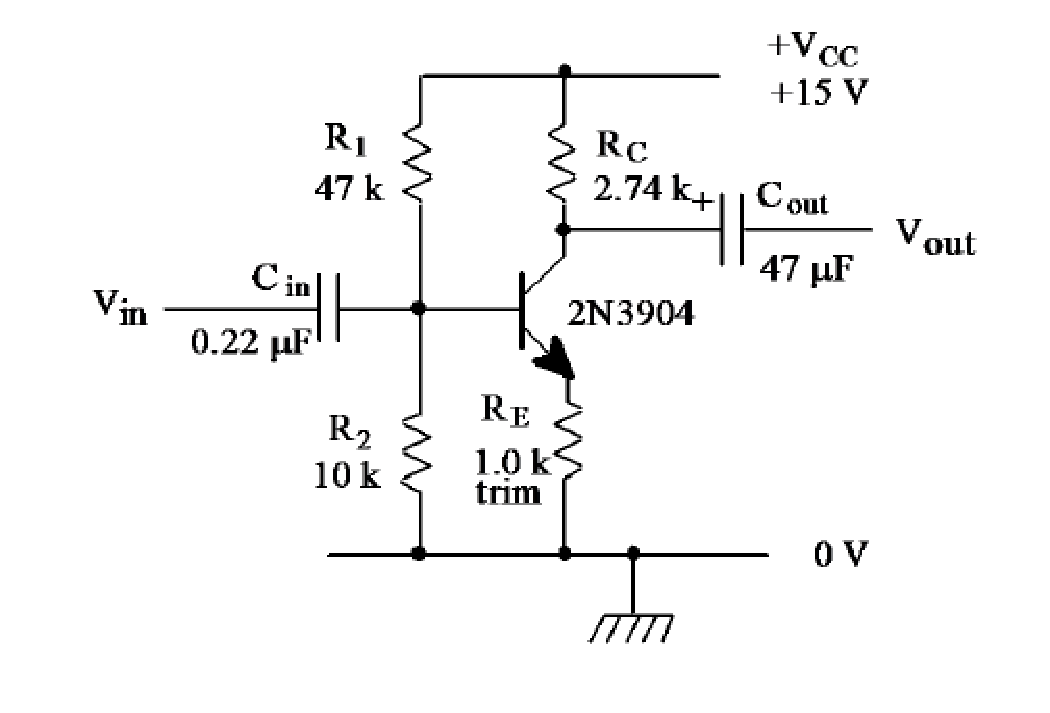
\includegraphics[scale=0.50]{EmitAmpSch.eps}
\caption{\textit{A schematic for the biased common emitter amplifier}}
\label{EmitAmp}
\end{figure}
We see that the input bias voltage, $V_B$, is given by the voltage divider made by $R_1$ and $R_2$. So we can calculate $V_B$ as
\begin{equation}
V_B = \frac{V_{CC}R_2}{R_1+R_2}
\label{BiasVolt}
\end{equation}
Now we know that emitter voltage is $0.6\unit{V}$ less than the bias voltage so
\begin{equation}
V_E = V_B - 0.6
\label{EmitVolt}
\end{equation}
The collector voltage $V_C$ is determined by the current through the collector so
$$V_C = V_{CC}-I_CR_C$$
but we assume that $I_E = I_C$ by neglecting the current through the bias. Using \emph{Ohm's Law} we can say that $I_E = V_E/R_E$ so we can find the collector voltage as
\begin{equation}
V_C = V_{CC} - \frac{V_E}{R_E}R_C
\label{CollVolt}
\end{equation}

The AC voltage gain of this circuit is given by
\begin{equation}
A = -\frac{R_C}{R_E+r_e}
\label{ACGain}
\end{equation}
where $r_e$ is the internal resistance of the emitter which is about $r_e = 12.5\unit{\Omega}$.

To now if we were to connect the wiper of the trim pot to the emitter end of the transistor (see figure \ref{EmitAmp2}) the gain becomes
\begin{equation}
A = -\frac{R_C}{r_e}
\label{GainPot}
\end{equation}
where $r_e$ is still the internal resistance of the emitter.


\section{Experiment}
To begin we found that the 2N3906 transistor is a pnp transistor by using a digital multimeter. We then found that the 2N3904 transistor was a npn transistor again by using the digital multimeter. 

Next we built a Biased Common Emitter Amplifier as shown in figure \ref{EmitAmp}. Where $R_C = 2.64\unit{k\Omega}$, $R_1=46.1\unit{k\Omega}$, $R_2=9.97\unit{k\Omega}$, $R_E = 0.929\unit{k\Omega}$, $C_{out} = 44.5\unit{\mu F}$, $C_{in} = 226\unit{nF}$, $C_E=45.2\unit{\mu F}$, and $C_B = 44.6\unit{\mu F}$. We connected the DC power supply so that $V_{CC} = +15\unit{V}$. We did not send any signal into the circuit so we could measure the quiescent voltages. Using a digital multimeter we found that $V_B = 2.54\unit{V}$, $V_E=1.87\unit{V}$, and $V_C=9.65\unit{V}$. Using equation \ref{BiasVolt} and the measured values of $R_1$ and $R_2$ we expect that $V_B=2.67\unit{V}$. So then equation \ref{EmitVolt} yields the expected value of $V_E=2.07\unit{V}$, and equation \ref{CollVolt} yields the expected value of $V_C=9.12\unit{V}$. Note that all the quiescent voltages agree within 10\%.

Next we hooked up the circuit to the oscilloscope using the $10\times$ probe. Then we sent an input signal in the form of a sine wave with a frequency of $10\unit{kHz}$. We then varied the amplitude of the sine wave until we saw clipping. Or at higher voltages when the circuit could not draw anymore power from the DC power supply and the circuit railed. We found that the largest output signal we got before clipping began was at $11.4\unit{V_{pp}}$.

Next we measured the gain at about half of the maximum level. Using the cursors on the oscilloscope we found that $V_{in} = 2.02\unit{V_{pp}}$ and $V_{out} = 5.84\unit{V_{pp}}$ these values give us a gain of $A = -2.89$. Note that the value is negative due to the fact that the output signal is inverse of the input. Now if can find the predicted value of $A$ by using equation \ref{ACGain} and the measured values $R_C = 2.64\unit{k\Omega}$ and $R_E = 0.929\unit{k\Omega}$. We calculate the expected value of $A$ as $A = -2.80$. So our measured gain agrees with the predicted gain.

After we verified the gain of the circuit made sense we connected the wiper of the trim pot $R_E$ through the bypass capacitor $C_E$ to ground as shown in figure \ref{EmitAmp2}.
\begin{figure}[h]
\centering
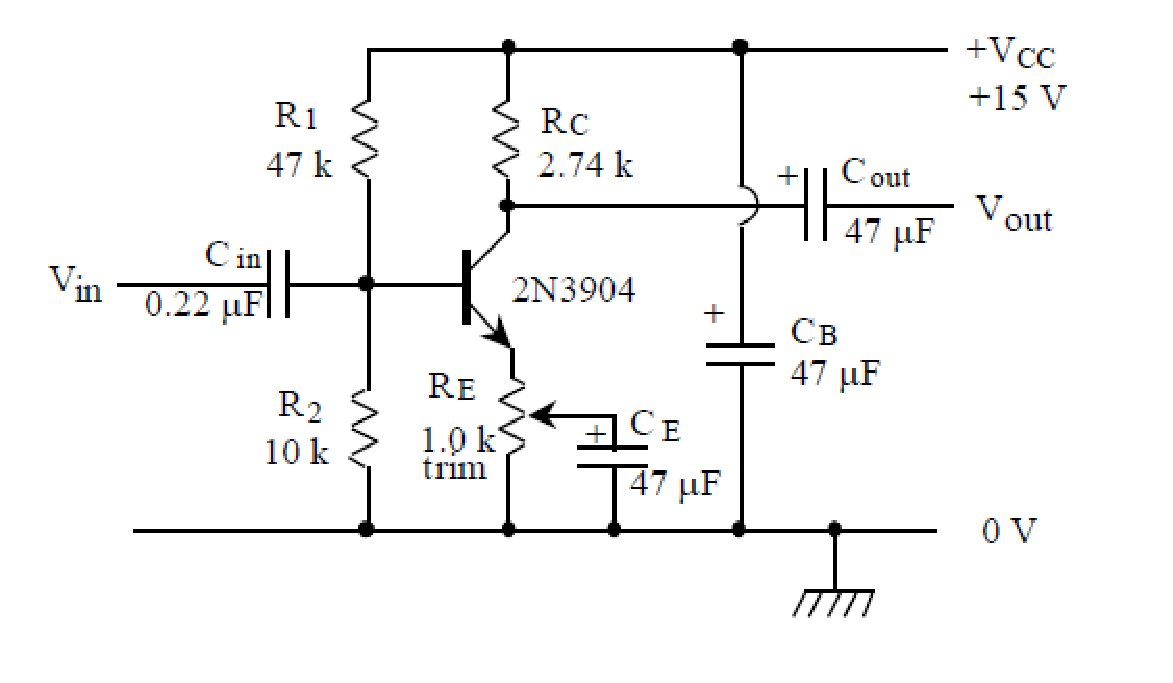
\includegraphics[scale=0.50]{EmitAmpSch2.eps}
\caption{\textit{A schematic for the biased common emitter amplifier, with variable gain}}
\label{EmitAmp2}
\end{figure}
 This allowed us to change the gain of the circuit by changing the resistance through the wiper. First though we had to lower the input signal. The function generator's lowest amplitude is $100\unit{mV}$ and this is not low enough for the gains we will get. So we attached a resistor (measured at $4.90\unit{\Omega}$) to ground in parallel with the input signal. We then measured the input and output voltage to measure the gain at different points (see table \ref{MaxGainTab}).
\begin{table}[h]
\centering
\begin{tabular}{ccc}
$V_{in}$	&$V_{out}$	&Gain ($A$)\\
\hline
$26.8\unit{mV}$	&$4.68\unit{V}$	&$175$\\
$18.1\unit{mV}$	&$3.24\unit{V}$	&$180$\\
$9.4\unit{mV}$	&$1.61\unit{V}$	&$171$\\
\end{tabular}
\caption{\textit{The gain of different input amplitudes going down by a factor of 2.}}
\label{MaxGainTab}
\end{table}
Now from equation \ref{GainPot} and the measured value $R_C=2.64\unit{k\Omega}$ we find that we expect the gain to be $A=-211$. We see that we did not account for the full internal resistance of the emitter as we assumed that $r_e=12.5\unit{\Omega}$ this accounts for the lower gain in the lab than we expected.

Next we want to find the resistance through the trim pot $R_{E1}$ that will give us a gain of $A=-25$. To do this we measured an input voltage of $18.0\unit{mV}$ (note that we kept the resistor in to keep our input voltages low) and we adjusted the trim pot until we had an output voltage that was 25 times our input or $V_{out} = 450\unit{mV}$. Once we got the output voltage we wanted we removed the trim pot and measured the resistance of $R_{E1}$ using a digital multimeter. We measured $R_{E1} = 90.2\unit{\Omega}$. Now we see that if we solve equation \ref{ACGain} for $R_E$ with $A=-25$ we can find the expected value of $R_{E1}$. Using $R_C=2.64\unit{k\Omega}$ we found the expected value of $R_{E1}$ as $R_{E1} = 93.1\unit{\Omega}$. This agrees with the value we measured.

To test the effect of input impedance on this circuit we connected a resistor (measured as $995\unit{\Omega}$ in series with the input signal. This resistor will simulate an input impedance. Once we did this we measured the output voltage as $V_{out} = 27.2\unit{mV}$. Note that the output voltage before was $V_{out0}=450\unit{mV}$. So we can see that by adding the input impedance we scaled the output voltage down by a factor of $0.060$ or $V_{out} = 0.060V_{out0}$. 

We then tested the effect of the output impedance on the circuit by removing the resistor we just put in and then connecting a $557\unit{\Omega}$ resistor to ground in parallel with the output signal. We found that the output voltage dropped to $V_{out}=83.0\unit{mV}$. We can find the expected value of this output voltage by using 
\begin{equation}
V_{out} = V_C\frac{R}{r_{out}+R}
\label{Imp}
\end{equation}
Where $V_C$ is the collector voltage measured as $V_C=9.65\unit{V}$, $R$ is the load impedance measured as $R=557\unit{\Omega}$, and $r_{out}$ is the output impedance of the circuit given as $r_{out} = 2.74\unit{k\Omega}$. Equation \ref{imp} implies that the output voltage will scale down a factor of $R/(R+r_{out})$ which we calculated as $0.170$. Now we measured $V_{out}$ as $83.0\unit{mV}$ with the impedance. This output voltage dropped down from $V_{out0} = 450\unit{mV}$. So the fraction of the original output voltage was $V_{out} = 0.184V_{out0}$. This value is close to our expected value.

\section{Conclusion}
In this lab we learned about the amplifying properties of a npn transistor. We found that we can create a more stable amplifier without needing any feedback. And by using a potentiometer we can change the gain of the circuit this will be useful for when we want to change the output signal by a specific amount.


\end{document}

